\documentclass[a4paper,12pt]{report}

\usepackage[utf8]{inputenc} % vagy latin2 helyett utf8
\usepackage[T1]{fontenc}      % karakterkódolás
%\usepackage[magyar]{babel}    % magyar beállítások
\frenchspacing                % helyközök
%\usepackage{times}           % betûtípus
\usepackage{lmodern}          %   vagy inkább ez

\usepackage[margin=2.5cm,left=3.5cm,includeheadfoot]{geometry}
                              % margók
\usepackage{graphicx}         % képekhez
\usepackage{setspace}         % sorköz
\onehalfspacing               % másfeles

\begin{document}

% ------------------------------------------------------------------------------
% Címlap

\begin{titlepage}

\noindent
\parbox[m]{0.2\textwidth}{
    
\includegraphics[width=0.2\textwidth]{img/elte_logo_colored.eps}
}
\hfill
\parbox[m]{0.7\textwidth}{
    \begin{center}
    \begin{large}
    \textsc{
        Eötvös Loránd University\\
        \vspace{0.5pc}
        Faculty of Informatics\\
        \vspace{0.5pc}
        Department of Programming Languages and Compilers\\
    }
    \end{large}
    \end{center}
}

\vspace{1pc}
\hrule

\vfill

\begin{center}
    {\LARGE Tool support for C++ template metaprogramming}
\end{center}

\vfill

\noindent
\hspace*{0.05\textwidth}
\parbox{0.45\textwidth}{
    {\it Supervisor:}
    \bigskip

    {\Large Zoltán Porkoláb}
    \smallskip

    Associate Professor
}
\hfill
\parbox{0.45\textwidth}{
    {\it Author:}
    \bigskip

    {\Large András János Kucsma}
    \smallskip

    Software Information Technology BSc
}


\vfill

\begin{center}
    {\large {\it Budapest, 2014}}
\end{center}

\end{titlepage}


% ------------------------------------------------------------------------------
% Témabejelentõ

\vspace*{\fill}
\begin{center}
Temabejelento
\end{center}
\vfill
\thispagestyle{empty}
\newpage
\setcounter{page}{1}

\tableofcontents

% TODO maybe \include is better?
% http://en.wikibooks.org/wiki/LaTeX/Modular_Documents#Getting_LaTeX_to_process_multiple_files

\chapter{Introduction}

\section{Motivation}

\section{Problem definition}

\section{Results} % what has been done

\section{Structure} % TODO find better word for this



% Maybe some stuff about template metaprogramming in this chapter?

\chapter{User documentation}

\section{Target audience}

This document expects the reader to have a basic understanding of template
metaprogramming in C++.

\section{Main concepts}

\section{Installation}

Metashell supports all major operating systems. In this section, installation
instructions only for Linux is described.

\subsection{Dependencies}

Install the dependent libraries and tools:

\begin{itemize}
    \item Readline
    \item Termcap
    \item CMake
\end{itemize}

Build Clang with Templight\cite{templight}:

\begin{itemize}
    \item \lstinline$mkdir build$
    \item \lstinline$cd build$
    \item \lstinline$cmake ../llvm -DLIBCLANG_BUILD_STATIC=ON$
    \item \lstinline$make clang$
    \item \lstinline$make libclang$
    \item \lstinline$make libclang_static$
\end{itemize}

\subsection{Building}

Now compile Metashell. In the source directory run the following commands:

\begin{itemize}
    \item \lstinline$mkdir bin$
    \item \lstinline$cd bin$
    \item \lstinline$cmake ..$
    \item \lstinline$make$
\end{itemize}

\subsection{Running tests}

To make sure everything will work correctly, running tests is advised:

\begin{itemize}
    \item \lstinline$test/metashell_test$
\end{itemize}

\section{Basic Usage}

%TODO how to start the program: ./app/metashell

\section{Command reference}

In the following section, the following notations are used: command parameters
that are in square brackets are optional. Parameters that are between angle
brackets have to be replaced by the user with something.

\subsection{evaluate}

Usage: \verb$evaluate [-full] [<type>]$

Evaluate and start debugging a new metaprogram.

Evaluating a metaprogram using the \verb$-full$ qualifier will expand all
Memoization events.

If called without <type>, then the last evaluated metaprogram will be
reevaluated.

Previous breakpoints are cleared.

Unlike metashell, evaluate doesn't use metashell::format to avoid cluttering
the debugged metaprogram with unrelated code. If you need formatting, you can
explicitly enter \verb$metashell::format< <type> >::type$ for the same effect.

\subsection{step}

Usage: \verb$step [over] [n]$

Step the program.

Argument n means step n times. n defaults to 1 if not specified.
Negative n means step the program backwards.

Use of the \verb$over$ qualifier will jump over sub instantiations.

\subsection{rbreak}

Usage: \verb$rbreak <regex>$

Add breakpoint for all types matching \verb$<regex>$.



\subsection{continue}

Usage: \verb$continue [n]$

Continue program being debugged.

The program is continued until the nth breakpoint or the end of the program
is reached. n defaults to 1 if not specified.
Negative n means continue the program backwards.

\subsection{forwardtrace}

Usage: \verb$forwardtrace|ft [n]$

Print forwardtrace from the current point.

The n specifier limits the depth of the trace. If n is not specified, then the
trace depth is unlimited.

\subsection{backtrace}

Usage: \verb$backtrace|bt $

Print backtrace from the current point.



\subsection{help}

Usage: \verb$help [<command>]$

Show help for commands.

If <command> is not specified, show a list of all available commands.

\subsection{quit}

Usage: \verb$quit $

Quit metadebugger.








\chapter{Developer documentation} \label{devdoc}

\section{Implementation plan}

\subsection{Internal workings}

At the start of the implementation of Metadebugger the following tools were
already implemented:
\begin{description}
    \item[Metashell]\cite{github} \hfill \\
        Metashell at version 1.0.0 \cite{github-releases} could already
        interactively evaluate metaprograms using the Clang\cite{clang}
        compiler through the libclang\cite{libclang} interface as its backend.
    \item[Templight]\cite{templight} \hfill \\
        Templight is a source code patch to Clang, which modifies the code
        of the template instantiation process of the compilation, so that it can
        produce a trace of the template instantiation process.
\end{description}

The trace generated by Templight then can be used to build a call graph for the
evaluated metaprograms. Traversing this call graph in a depth first manner is
what the compiler did while evaluating the entered metaprogram. This means,
that we can debug a template metaprogram after it has been compiled, thus
completely avoiding the complications that can arise if we stop or suspend the
compiler in the middle of the compilation process.

\pagebreak

Here is a diagram showing this architecture:

\begin{figure}[H]
    \centering
    
\begin{tikzpicture}[auto, node distance=2cm,>=latex']
    \tikzstyle{block} = [draw, rectangle, text centered];
    \tikzstyle{metashell-block} = [draw, rectangle, inner sep=0.2cm];
    \tikzstyle{clang-templight-block} = [draw, rectangle, inner sep=0.2cm];
    \node [block, text width=2.1cm]
        (templight)
        {Templight};
    \node [above=0.2cm of templight]
        (clang)
        {Clang};
    \node [clang-templight-block, fit = (templight) (clang)]
        (clang-templight)
        {};
    \node [block, below=2cm of clang-templight, text width=2.5cm]
        (trace)
        {Template instantiation trace};
    \node [block, left=2cm of clang-templight, text width=2.5cm]
        (cpp-code)
        {Entered C++ code};
    \node [block, left=2cm of trace, text width=2.5cm]
        (metadebugger)
        {Metadebugger};
    \node [above=0.2cm of cpp-code]
        (metashell)
        {Metashell};
    \node [metashell-block, fit = (cpp-code) (metadebugger) (metashell)]
    {};

    \path[draw,->]
    (cpp-code) edge (clang-templight)
    (templight) edge (trace)
    (trace) edge (metadebugger);
\end{tikzpicture}

    \caption{Architecture plan}
\end{figure}

\subsection{Interface}

Most of the C++ programmers are familiar with gdb\cite{gdb} and its command
line interface, so it was natural to choose an interface plan similar to gdb's
in order to lower the learning curve for the new users of Metadebugger.

\section{Algorithms and data structures used}

\subsection{The representation of a metaprogram}

%Mihalicza: page 69
C++ template metaprogramming can be seen as a form of purely functional
programming\cite{mihalicza-phd}. In functional programming a program's main
components are the functions. In metaprogramming, functions are represented by
so called metafunctions. Metafunctions are basically templated structs or
classes, which get their parameters as template parameters, and return values
by defining member types or compile time constants based on the template
parameters. There is actually a more strict
definition\cite{boost-mpl-metafunction} of metafunction by the developers of
Boost MPL library\cite{boost-mpl}. For our purposes the loose definition above
will suffice.

For a specific metaprogram, Metadebugger represents only the metaprogram's call
graph. For example instantiating \texttt{int\_<fib<5>::value>} would be
represented by the following graph in Metadebugger:

\begin{figure}[H]
    \includegraphics[width=\textwidth]{img/fib5_call_graph.eps}
    \caption{Internal representation of the fibonacci metaprogram}
\end{figure}

\noindent
It can be seen from the above figure, that the graph vertices represent types,
and edges represent instantiation events. A type can instantiate multiple
types, and a type can be referenced from multiple places. The first reference
to a type will be a TempateInstantiation event (as it is instantiated for the
first time by the compiler). The following references will reuse the already
created type, so those become Memoization events.

\subsection{Graph filtering} \label{graph-filtering}

The underlying C++ compiler emits a lot of instantiation events which don't
have real value to the user. These events need to be filtered out from the
graph for better user experience. The edges which represent these events are
not physically taken out from graph, only an edge property flag is set to
disable the edge. Algorithms which traverse the graph will of course have to
check this flag to operate only on the interesting part of the graph.

The decision to only use a flag instead of modifying the graph has the
following properties:

\begin{itemize}
    \item
        Faster filtering process, since the internal vectors used to represent
        the graph are not touched.
    \item
        Uses more memory, since memory used by unused data are not freed back
        to the operating system.
    \item
        Not currently implemented, but these unused parts of the graph can be
        enabled for the advanced users, if they're interested.
    \item
        In boost's graph implementation, \texttt{vertex\_descriptor}
        objects used to refer to vertices of the graph are unsigned integers.
        The documentation promises, that these \texttt{vertex\_descriptor}
        start from 0 and go up from there for every vertex added to the graph.
        The algorithms in Metadebugger relies heavily on this handy property.
        Removing vertices from the graph would break this continuous indexing.
\end{itemize}

The filtering process takes multiple stages. The filter algorithm starts out
with a graph, where all edges are enabled.

\begin{enumerate}
    \item
        Disable all edges. This is useful because the following stages become
        simpler.
    \item
        Enable edges going from the root vertex for which the
        \texttt{point\_of\_instantiation} edge property matches the currently
        entered line. This is to filter out instantiation sub trees, which were
        not initiated by the type entered by the user.
    \item
        Now a depth first traversal is done from the root vertex going only on
        the edges we enabled in the previous section. For every new vertex the
        traversal encounters, the algorithm enables all out edges, and
        continues the traversal through these edges.
    \item
        Clang generates a TemplateInstantiation and a Memoization event for the
        result type. Disable the Memoization one. In this process, the name of
        the vertex pointed by these two edges is trimmed too, so the
        \texttt{metashell::wrap} wrapper doesn't clutter the result.
    \item
        Clang sometimes triggers multiple Memoization events for the same type
        instantiated from a single type, and thus equivalent parallel edges
        appear in the graph. Since the user doesn't get any useful information
        about how many times Clang internally checked a type instantiation,
        these get filtered out as well.
\end{enumerate}

\subsection{Forwardtrace}

When at some point the user wants to see what will happen in the future with
the current type it is the easiest to issue a forwardtrace command. Here is
what the forwardtrace looks like from the very beginning of the evaluation of
\texttt{int\_<fib<5>::value}:

\bigskip

\begin{figure}[H]
    
\begin{tttenv}
(mdb) ft \\
int\_<fib<{\color{color04} 5}>::value> \\
{\color{color03} + }fib<{\color{color04} 5}> (TemplateInstantiation) \\
{\color{color03} \textbar{} }{\color{color06} + }fib<{\color{color04} 3}>
(TemplateInstantiation) \\
{\color{color03} \textbar{} }{\color{color06} \textbar{} }{\color{color07} + }fib<{\color{color04} 1}>
(Memoization) \\
{\color{color03} \textbar{} }{\color{color06} \textbar{} }{\color{color07} ` }fib<{\color{color04} 2}>
(TemplateInstantiation) \\
{\color{color03} \textbar{} }{\color{color06} \textbar{} }{\color{color07} \hspace{0.5em} }{\color{color08} +
}fib<{\color{color04} 0}> (Memoization) \\
{\color{color03} \textbar{} }{\color{color06} \textbar{} }{\color{color07} \hspace{0.5em} }{\color{color08} `
}fib<{\color{color04} 1}> (Memoization) \\
{\color{color03} \textbar{} }{\color{color06} ` }fib<{\color{color04} 4}>
(TemplateInstantiation) \\
{\color{color03} \textbar{} }{\color{color06} \hspace{0.5em} }{\color{color07} + }fib<{\color{color04} 2}>
(Memoization) \\
{\color{color03} \textbar{} }{\color{color06} \hspace{0.5em} }{\color{color07} ` }fib<{\color{color04} 3}>
(Memoization) \\
{\color{color03} + }fib<{\color{color04} 5}> (Memoization) \\
{\color{color03} ` }int\_<{\color{color04} 5}> (TemplateInstantiation) \\
\end{tttenv}

    \caption{Forwardtrace output example}
\end{figure}

\noindent
The algorithm which prints this is basically a depth first traversal printing
a line every time it is visiting a vertex. The algorithm is iterative and thus
keeps track of the edges it has to visit in a stack. In addition it also keeps
track of the current depth of the traversal in the stack, so the depth of the
indentation is known when printing a line.

For better readability, it is also required to know for every depth less than
the current depth if the algorithm should print a \texttt{'|'} or not. This
is achieved by having a vector of counters from 0 to the current depth. Each
element in the vector counts how many elements are there in the stack with that
particular depth. For every depth, the algorithm prints \texttt{'|'} when
this counter is greater than 0.

\subsection{Stepping}

The algorithm for basic stepping is very similar to forwardtrace: in it's core
it is also a depth first traversal of the underlying call graph. There are two
other extra things step has to be able to do:

\begin{enumerate}
    \item
        Stop at any point in the traversal, so the user can inspect the current
        state of the metaprogram.
    \item
        Going backwards in the traversal. This happens, when the user calls the
        step command with a negative argument.
\end{enumerate}

Stopping at any point was achieved by creating a \texttt{state\_t} structure
which describes the current state of the metaprogram. It was put in the
metaprogram class' scope, and a \texttt{void metaprogram::step()} function
was created which does a single iteration of the depth first traversal by
updating the state structure. The \texttt{state\_t} struct and the step
function:

\begin{figure}[H]
    \includecode{src/metaprogram_state_t.hpp}
    \caption{Code section describing \texttt{step()} and \texttt{state\_t}}
\end{figure}

\noindent
The other very useful feature of stepping is going backwards. The user can
achieve this by passing a negative argument to the \texttt{step} command. For
this the \texttt{void metaprogram::step\_back()} function was implemented which
also updates the state struct, but does the opposite of \texttt{step()}. This
means, that if \texttt{step()} was called from state A and resulted in state
B, then calling \texttt{step\_back()} from state B will result in state A.
The two endpoint states (when nothing has been discovered and when every
reachable vertex was discovered) are exceptions from this rule.

When step is executing, it marks the changes it made into the state into a
\texttt{rollback\_t} structure and pushes them onto a stack:

\begin{figure}[H]
    \includecode{src/metaprogram_rollback_t.hpp}
    \caption{Code section describing \texttt{step\_back()} and
        \texttt{rollback\_t}
    }
\end{figure}

\noindent
\texttt{step\_back()} simply picks pops the top element from the stack, and
restores the state change the last \texttt{step()} did, based on the
rollback structure.

\subsection{Command matching}

Users of any software will want to do a particular task with less and less
effort as they get more experience with the tool. For a command line tool like
Metadebugger, this need basically boils down to typing as few characters as
possible.

To aid this, an algorithm similar to gdb's command matching was implemented.

If the user enters a prefix of a command which uniquely identifies the command
(so there is no other command with that same prefix), than that command should
be executed. In Metadebugger some commands also have aliases (for example, a
shortened alias for the command \texttt{"backtrace"} is \texttt{"bt"}). The
entered command should also be accepted when it is not a prefix for a unique
command, but all possible candidate commands are aliases for the same command.
For example the input \texttt{"b"} should be accepted as a command for
backtrace, even though it is not a unique prefix.

Pseudocode for the algorithm:

\begin{figure}[H]
    \includecode{src/command_matching.cpp}
    \caption{The algorithm for command matching}
\end{figure}

\pagebreak

\section{Class hierarchy}

Here is the class diagram for the main classes that form the core components of
Metadebugger.

\begin{figure}[H]
    \centering
    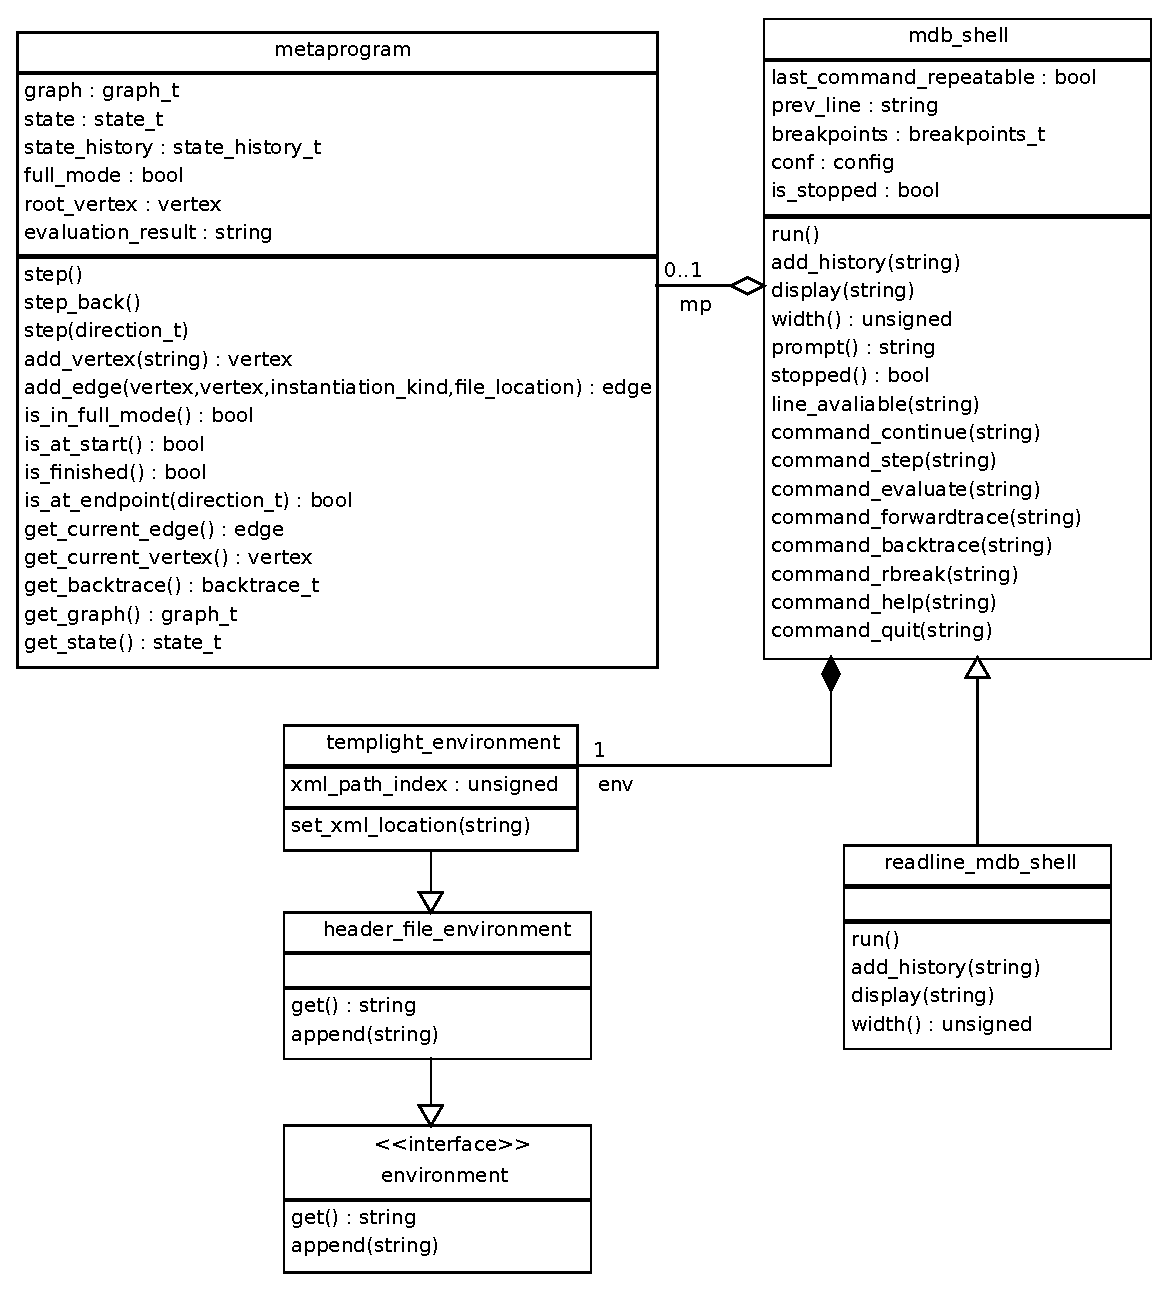
\includegraphics[width=\textwidth]{img/mdb_class_diagram.eps}
    \caption{Metadebugger class diagram}
\end{figure}

\noindent
Notes:
\begin{itemize}
    \item
        Only public member functions and private member variables are shown
        on the diagram.
    \item
        Lot of smaller, helper structures and classes are hidden.
    \item
        There is another class inheriting \texttt{mdb\_shell} called
        \texttt{mdb\_test\_shell}. This class is only used for testing
        purposes to mock out the actual shell and Readline related
        functionalities, which would make automated testing very difficult.
\end{itemize}

\section{Libraries used}

Several libraries are used by Metadebugger. In the section the main libraries
are listed.

\subsection{Boost}

Boost\cite{boost} is a set of open source C++ libraries that provide ready to
use solutions to common tasks. In Metadebugger several Boost libraries are
being used:
\begin{description}
    \item[Boost.Graph]\cite{boost-graph} \hfill \\
        This library provides a generic interface and implementations of graph
        data-structures and algorithms.

        In Metadebugger the information which is gathered by Templight is
        stored in a Boost.Graph data-structure. Since the whole program is
        revolving around the metaprogram which being debugged, it was very
        important to choose a robust and flexible graph library.
    \item[Boost.Optional]\cite{boost-optional} \hfill \\
        Unlike in some programming languages, in C++ stack allocated objects
        cannot have a null value. This have some advantages, for example the
        programmer doesn't have to check for a null value before doing
        operations on an object.

        But at the same time, sometimes it is useful to have an object state,
        in which the object is invalid in purpose. Boost.Optional provides an
        easy way to turn any type into a type which can have an invalid state
        called \texttt{boost::none}.
    \item[Boost.PropertyTree]\cite{boost-pt} \hfill \\
        The Boost.PropertyTree library provides a data structure that stores an
        arbitrarily deeply nested tree of values, indexed at each level by some
        key.

        Metadebugger makes use of the xml parsing capabilities of
        Boost.PropertyTree to parse the xml created by Templight.
    \item[Boost.Regex]\cite{boost-regex} \hfill \\
        Boost.Regex provides support for regular expressions in C++.

        Metadebugger uses regular expressions to match type names when
        breakpoints are used.
    \item[Boost.Filesystem]\cite{boost-fs} \hfill \\
        Boost.Filesystem provides a cross platform interface to manipulate the
        file system.

        Metadebugger uses Boost.Filesystem to create and delete the temporary
        file where the output of Templight is stored until it's processed.
    \item[Boost.StringAlgorithm]\cite{boost-string} \hfill \\
        Boost.StringAlgorithm provides a handful of useful string-related
        algorithms.

        Metadebugger has to manipulate strings in various contexts and makes
        use of a few algorithms contained in this library.
    \item[Boost.LexicalCast]\cite{boost-lexicalcast} \hfill \\
        Boost.LexicalCast provides an easy way to convert numbers to string
        form and the other way around.

        Metadebugger uses this library during parsing of the Templight xml
        file.

\end{description}

\subsection{Just}

Just\cite{just} is a collection of lightweight C++ libraries developed by
Sinkovics. The following Just libraries are used in Metadebugger:
\begin{description}
    \item[just::console] \hfill \\
        The just::console library provides a cross platform interface to output
        colored text to a console interface.

        Metadebugger uses colored text in its output for easier readability.
    \item[just::test] \hfill \\
        Just::test is a testing library.

        Metadebugger uses just::test to create unit and integration test cases.
\end{description}

\subsection{Clang}

Clang\cite{clang,libclang} is a C++ front end for LLVM. Together they form a
highly customizable C++ compiler. Clang is used to compile the source code
given as an input to Metadebugger.

\subsection{Templight}

Templight\cite{templight} (in its current form) is a source code patch to
Clang. With Templight, Clang is able to generate a trace about the template
instantiation steps during compilation. Metadebugger takes this output and
creates the necessary data structures to be able to simulate the compilation.

\subsection{Readline}

The Readline library\cite{readline} is the de facto standard library used to
handle user inputs in software that uses an interactive command line interface.



\begin{thebibliography}{9}
\bibitem{v} Valaki, valami.
\end{thebibliography}

\end{document}
